\documentclass{standalone}
\usepackage{tikz}
\usepackage{ctex,siunitx,ninecolors}
\setCJKmainfont{Noto Serif CJK SC}
\usepackage{tkz-euclide}
\usepackage{amsmath}
\usepackage{wasysym}
\usetikzlibrary{patterns, calc}
\usetikzlibrary{decorations.pathmorphing, decorations.pathreplacing, decorations.shapes}
\begin{document}
\small
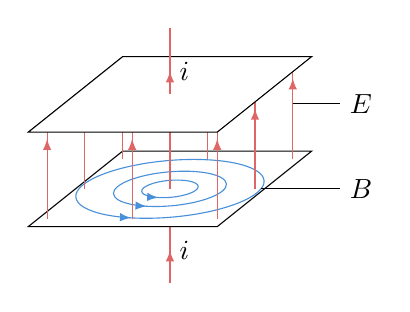
\begin{tikzpicture}[>=latex,scale=1.2]
  \draw[red6,postaction={decorate},decoration={markings,mark={at position 0.35 with {\arrow{>}}}}](0,-1)--(0,0)node[pos=0.35,right,text=black]{$i$};
  \draw[fill=white](-0.5,0.4)--++(-1,-0.8)--++(2,0)--++(1,0.8)--cycle;
  \draw[rotate=5,azure6,decoration={markings,mark={at position 0.65 with {\arrow{>}}}},postaction={decorate}](0,0)ellipse(0.3 and 0.09);
  \draw[rotate=5,azure6,decoration={markings,mark={at position 0.65 with {\arrow{>}}}},postaction={decorate}](0,0)ellipse(0.6 and 0.18);
  \draw[rotate=5,azure6,decoration={markings,mark={at position 0.65 with {\arrow{>}}}},postaction={decorate}](0,0)ellipse(1 and 0.3);
  \foreach \x in {-0.9,0,0.9}
  {
    \foreach \y in {-0.4,0,0.4}
    {
      \draw[red6,decoration={markings,mark={at position 0.85 with {\arrow{>}}}},postaction={decorate}](\x+\y,\y*0.8)--++(0,1.0);
    }
  }
  \draw[fill=white](-0.5,1.4)--++(-1,-0.8)--++(2,0)--++(1,0.8)--cycle;
  \draw[red6,postaction={decorate},decoration={markings,mark={at position 0.35 with {\arrow{>}}}}](0,1)--++(0,0.7)node[pos=0.35,right,text=black]{$i$};
  \draw[thin](0.96,0)--(1.8,0)node[right]{$B$};
  \draw[thin](1.3,0.9)--(1.8,0.9)node[right]{$E$};
\end{tikzpicture}
\end{document}